\documentclass{article}%
\usepackage[T1]{fontenc}%
\usepackage[utf8]{inputenc}%
\usepackage{lmodern}%
\usepackage{textcomp}%
\usepackage{lastpage}%
\usepackage[head=40pt,margin=0.5in,bottom=0.6in]{geometry}%
\usepackage{graphicx}%
%
\title{\textbf{Frente Amplio Nacional: Más de 1.700 propuestas se concretaron en congresos regionales}}%
\author{CRISBEL VARELA}%
\date{20/11/2018}%
%
\begin{document}%
\normalsize%
\maketitle%
\textbf{URL: }%
http://www.eluniversal.com/politica/26262/frente{-}amplio{-}nacional{-}mas{-}de{-}1739{-}propuestas{-}se{-}concretaron{-}en{-}congresos{-}regionales\newline%
%
\textbf{Periodico: }%
EU, %
ID: %
26262, %
Seccion: %
politica\newline%
%
\textbf{Palabras Claves: }%
NO\_TIENE\newline%
%
\textbf{Derecho: }%
12%
, Otros Derechos: %
NO\_TIENE%
, Sub Derechos: %
NO\_TIENE%
\newline%
%
\textbf{EP: }%
SI\newline%
\newline%
%
\textbf{\textit{Ángel Oropeza, miembro de la organización política, indicó que "el mensaje es que la gente quiere salir de esta tragedia y quiere organizarse para cumplir con el país que viene"}}%
\newline%
\newline%
%
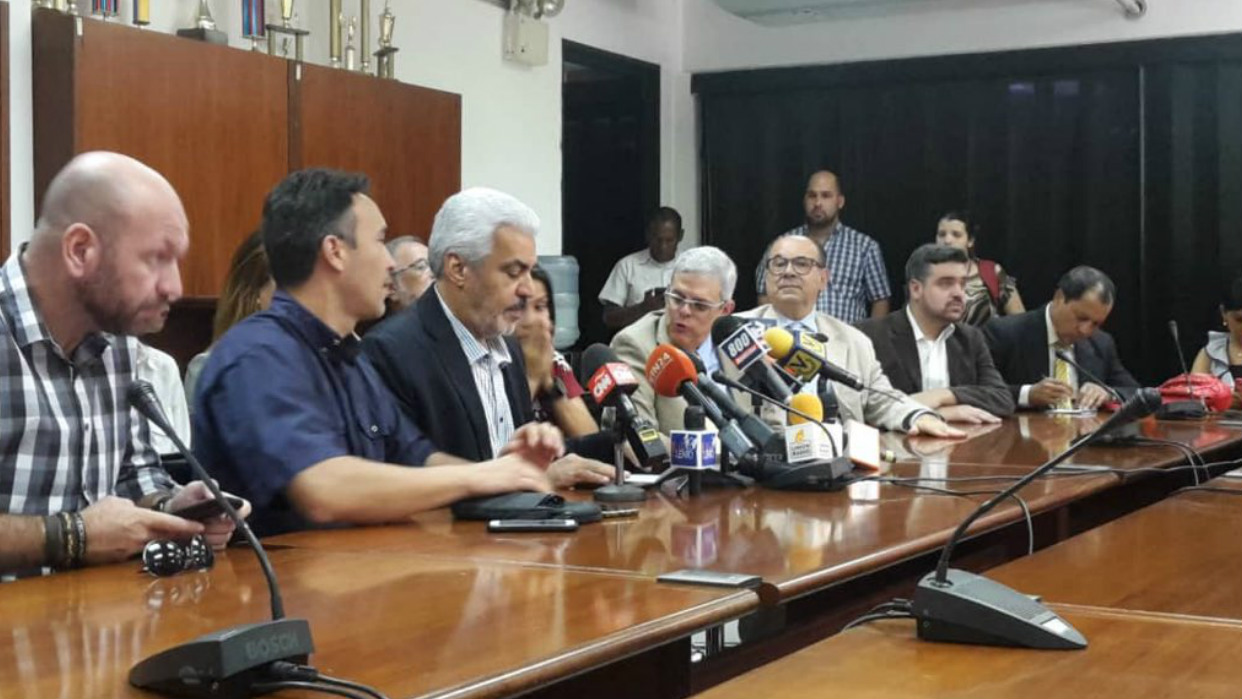
\includegraphics[width=300px]{22.jpg}%
\newline%
%
Caracas.{-} El Frente Amplio Nacional ofreció un balance sobre las asambleas regionales realizadas de cara al denominado "Congreso Nacional Venezuela Libre" que se tiene previsto para el próximo 23 de noviembre.%
\newline%
%
Ángel Oropeza, miembro de la organización política, precisó que hasta el momento tienen contabilizadas más de 1.739 propuestas, sin embargo, destacó que aún falta cuatro estados.%
\newline%
%
“De las mesas más concurridas fue la de estrategia y acciones de lucha y la segunda la de desarrollo local y nacional. El mensaje es que la gente quiere salir de esta tragedia y quiere organizarse para cumplir con el país que viene”, resaltó.%
\newline%
%
Oropeza explicó que estaban esperando 144 mesas, pero al final se instalaron 245.%
\newline%
%
\end{document}